% !TeX program = xelatex

\documentclass[
    aspectratio=169,
]{beamer}

\usepackage{minted}
\usepackage{todonotes}
\usepackage{makecell}

\usetheme{gray-scott}

\AtBeginSection{
    \begin{frame}{Outline}
        \renewcommand{\baselinestretch}{0.25}
        \tableofcontents[currentsection]
    \end{frame}
}

\setminted{
    autogobble,
    fontsize=\small,
    xleftmargin=0.5em,
    xrightmargin=0.5em,
    breaklines,
    style=nord,
    bgcolor=black,
    formatcom=\color{white},
}

\setminted[text]{
    fontsize=\scriptsize,
}

% Captions
% Captions
\renewcommand{\caption}[1]{%
    \begin{center}
        \color{darkgray}
        \scriptsize #1
    \end{center}%
}

\graphicspath{{images/}}

%Information to be included in the title page:
\title{Kokkos on CPU}
\subtitle{Gray-Scott School 2026}
\author{Mathieu Lobet, Paul Zehner, Paul Gannay, Hariprasad Kannan, Thomas Padioleau, Trévis Morvany}
\institute{CEA}
\date{2026-06-25}
\closing{%
    \begin{description}[\hspace{0.355\linewidth}]
        \item[Next Kokkos session] Thursday 2\textsuperscript{nd} of July for Kokkos on GPU
        \item[Kokkos website] \href{https://kokkos.org}{\texttt{kokkos.org}}
        \item[Kokkos repository] \href{https://github.com/kokkos}{\texttt{github.com/kokkos}}
        \item[Gray-Scott Kokkos repository] \href{https://github.com/Maison-de-la-Simulation/gray-scott-kokkos}{\texttt{github.com/Maison-de-la-Simulation/} \texttt{gray-scott-kokkos}}
    \end{description}
}

\begin{document}

\begin{frame}[plain]
    \titlepage
\end{frame}

\begin{frame}{About this course}
    \begin{columns}
        \begin{column}{0.5\linewidth}
            \begin{enumerate}
                \item CPU course (today!)
                \item GPU course (Thursday the 2\textsuperscript{nd})
            \end{enumerate}
        \end{column}
        \pause
        \begin{column}{0.5\linewidth}
            \begin{alertblock}{Caution}
                You need to attend the 2 courses to master Kokkos!
            \end{alertblock}
        \end{column}
    \end{columns}
\end{frame}

\begin{frame}{Outline}
    \renewcommand{\baselinestretch}{0.5}
    \tableofcontents
\end{frame}

\section{Introduction to Kokkos}

\begin{frame}{Performance, portability and productivity}
    \begin{columns}[T]
        \begin{column}{0.45\linewidth}
            \begin{center}
            \textbf{What \emph{most developers} want}
            \end{center}
            \begin{description}[Performance]
                \item[Performance] Get the best performance on a specific hardware
                \item[Portability] Run the same code on different hardware
                \item[Productivity] Write code quickly and easily, maintain and extend code, leverage architecture optimization
            \end{description}
        \end{column}
        \pause
        \begin{column}{0.55\linewidth}
            \begin{center}
                \textbf{What \emph{developers for science} also want}
            \end{center}
            \begin{description}[Interporability]
                \item[Maturity] Production-ready (i.e. not research product)
                \item[Community] Contributors, support, documentation, examples
                \item[Longevity] Long-term maintenance, bug fixes, updates, sponsorship
                \item[Interporability] Possibility to easily couple with other libraries and tools (IO, Linear Algebra, Machine Learning, etc.)
            \end{description}
        \end{column}
    \end{columns}
\end{frame}

\begin{frame}{Do \emph{you} need performance portability?}
    \begin{columns}[T]
        \begin{column}{0.6\linewidth}
            \begin{center}
                \textbf{Probably \emph{yes} if you...}
            \end{center}
            \begin{itemize}
                \item Want your code to run on different hardware technologies (CPU, GPU)
                \item Have performance requirements
                \item Cannot afford to maintain and optimize different versions of your code for each possible hardware of the market
                \item Want to focus on algorithmic and not on code development
                \item Want your code to be easily maintainable and readable by others, especially non experts
            \end{itemize}
        \end{column}
        \pause
        \begin{column}{0.4\linewidth}
            \begin{center}
                \textbf{Probably \emph{no} if you...}
            \end{center}
            \begin{itemize}
                \item Need to tune your algorithms to work as fast as possible on a given hardware
                \item Want to explore a new architecture
            \end{itemize}
        \end{column}
    \end{columns}
\end{frame}

\begin{frame}{Programming models }
    \begin{center}
        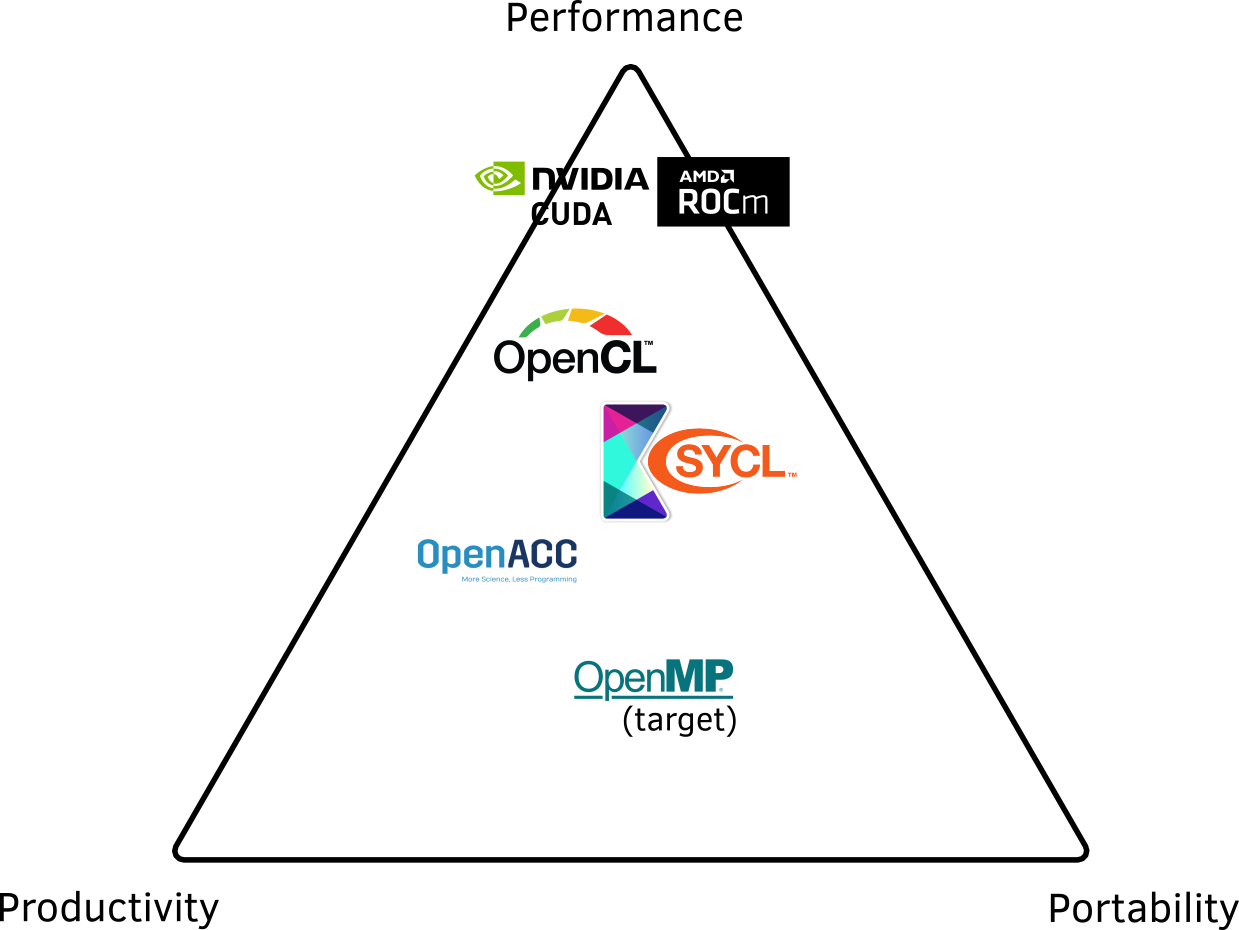
\includegraphics[width=0.5\textwidth]{p3.png}
    \end{center}
\end{frame}

\begin{frame}{Kokkos programming model}
    Kokkos is a performance portability parallel programming model built upon the C++-20 standard, designed to abstract already existing parallel programming models

    \vspace{0.5em}

    \begin{center}
        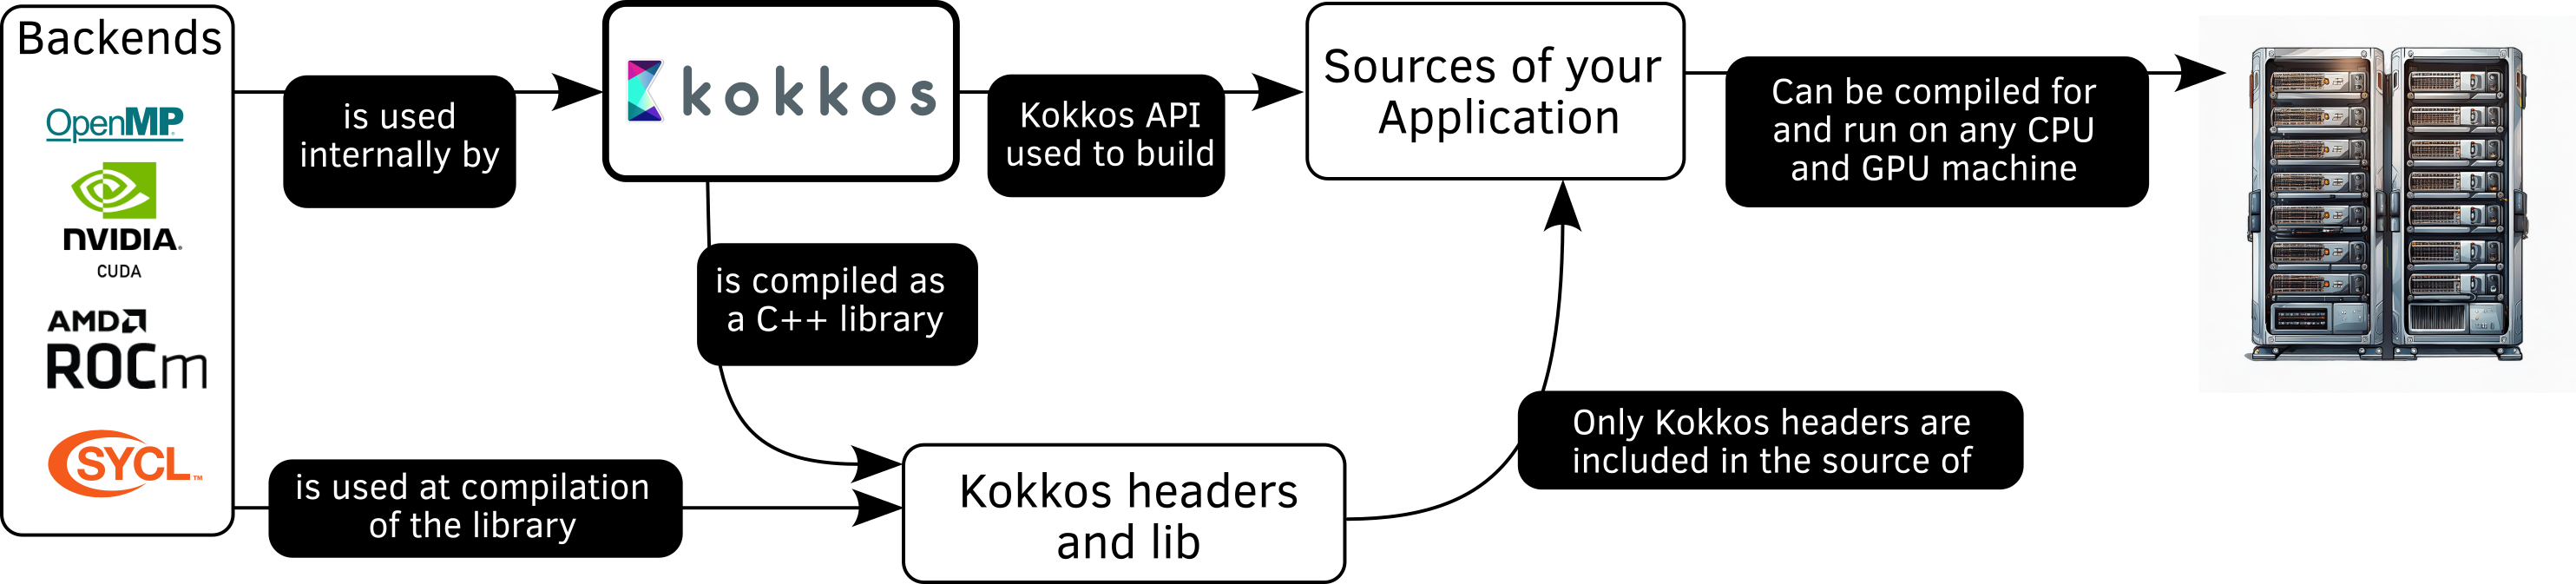
\includegraphics[width=0.9\textwidth]{kokkos_model.png}
    \end{center}
    \begin{itemize}
        \item Kokkos provides data structures and functions based on modern C++ to build your application
        \item Developers never directly use underlying backends (no Cuda kernels for instance)
    \end{itemize}
\end{frame}

\begin{frame}{Kokkos parallelism scope}
    \begin{itemize}
        \item Kokkos only handles node-level parallelism
        \item You still need a model for distributed memory parallelism (e.g.\ MPI, Kokkos-Comm)
    \end{itemize}
\end{frame}

\begin{frame}{What Kokkos provides you}
    \begin{itemize}
        \item Kokkos' basic capabilities
        \begin{itemize}
            \item Abstraction of most parallel patterns used in HPC (loops, reduction, scan)
            \item Abstracted basic data structures used in science (vectors, multidimensional arrays, sub-arrays, strided arrays, etc)
        \end{itemize}
        \pause
        \item Kokkos' advanced capabilities
        \begin{itemize}
            \item Advanced data structure properties
            \item Thread safety, thread scalability, and atomic operations
            \item Hierarchical patterns for maximizing parallelism
        \end{itemize}
        \pause
        \item Kokkos' libraries
        \begin{itemize}
            \item Profiling, tuning and debugging tools (Kokkos tools)
            \item Python and Fortran interfaces (PyKokkos, Kokkos-Fortran-interop)
            \item Linear algebra (Kokkos-Kernels)
            \item FFT (Kokkos-FFT)
            \item Distributed memory parallelism (Kokkos-Comm)
        \end{itemize}
    \end{itemize}
\end{frame}

\begin{frame}{Kokkos ecosystem}
    \begin{center}
        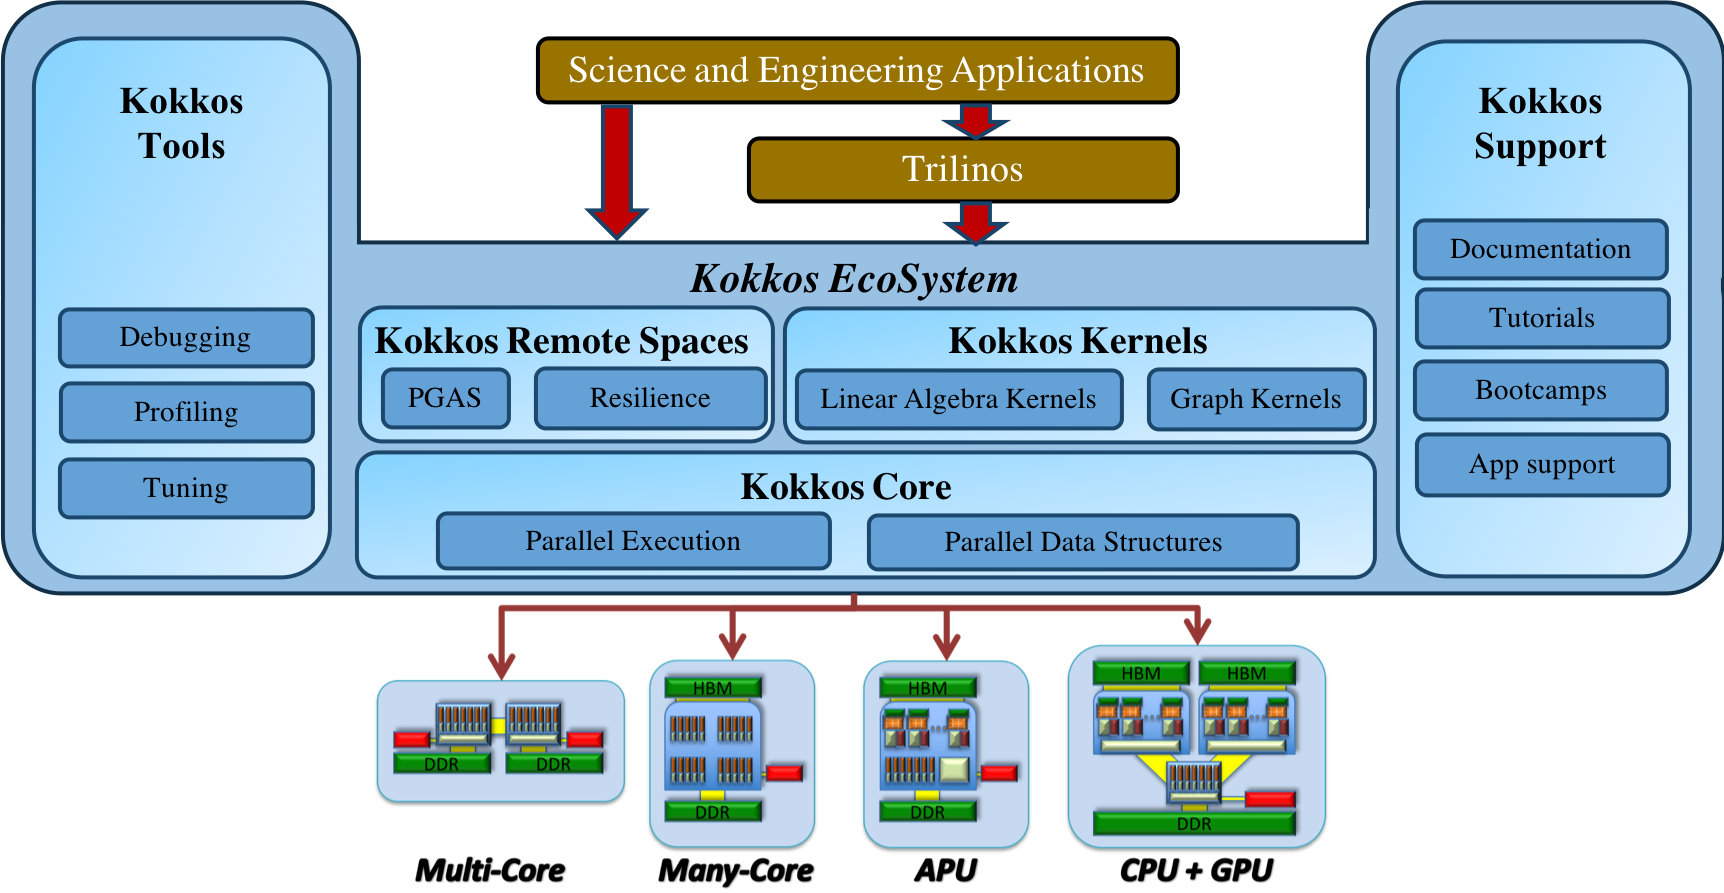
\includegraphics[width=0.9\textwidth]{kokkos-ecosystem.png}
    \end{center}
\end{frame}

\begin{frame}{Kokkos and the evolution of the C++ standard}
    \begin{center}
        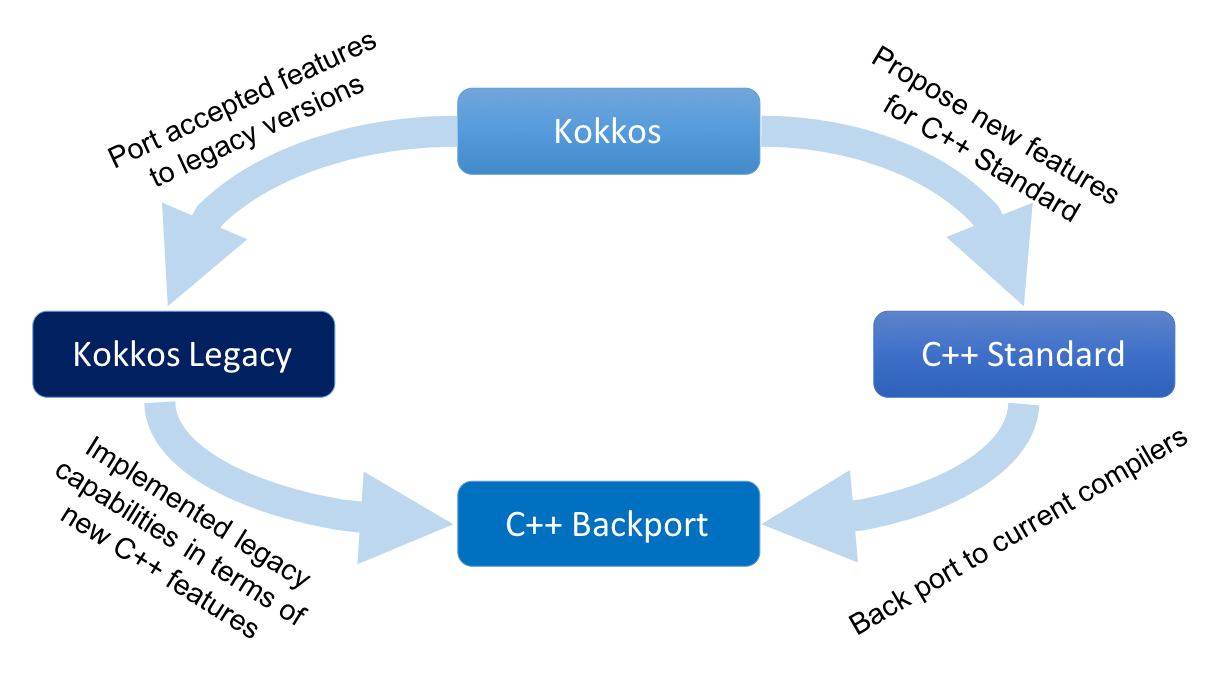
\includegraphics[width=0.9\textwidth]{kokkos-cpp-standard.png}
    \end{center}
\end{frame}

\begin{frame}{Kokkos history and governance}
    \begin{columns}
        \begin{column}{0.45\linewidth}
            \centering

            
\includegraphics[width=0.6\linewidth]{hpsf}

            \vspace{2em}

            
\includegraphics[width=0.8\linewidth]{kokkos_text}
        \end{column}
        \begin{column}{0.55\linewidth}
            \begin{itemize}
                \item Kokkos was initially developed in American laboratories in 2011
                \item Kokkos is a project of the High Performance Software Foundation (HPSF, part of the Linux Foundation) since 2023
                \item Not a purely American project anymore
                \item Sustainability of the development for the long run
            \end{itemize}
        \end{column}
    \end{columns}
\end{frame}

\begin{frame}{Kokkos useful resources}
    \begin{description}[GitHub repository]
        \item[GitHub repository] \url{https://github.com/kokkos}
        \item[Documentation] \url{https://kokkos.org/kokkos-core-wiki}
        \item[Slack channel] \url{https://kokkosteam.slack.com}
        \item[Cheat sheet] \url{https://cexa-project.org/documents}
    \end{description}
\end{frame}

\section{Docker images}

\begin{frame}{Docker images (CPU images)}
    \begin{itemize}
        \item No editor (\texttt{x86\_64}, \texttt{aarch64})

        {\tiny \url{gitlab-registry.in2p3.fr/thomas.padioleau/gray-scott-kokkos/kokkos_cpu_interactive:latest}}
        \item Jupyter (\texttt{x86\_64}, \texttt{aarch64})

        {\tiny \url{gitlab-registry.in2p3.fr/thomas.padioleau/gray-scott-kokkos/kokkos_cpu_interactive_jupyter:latest}}
        \item VSCode (\texttt{x86\_64}, \texttt{aarch64})

        {\tiny \url{gitlab-registry.in2p3.fr/thomas.padioleau/gray-scott-kokkos/kokkos_cpu_interactive_vscode:latest}}
        \item CodeServer (\texttt{x86\_64}, \texttt{aarch64})

        {\tiny \url{gitlab-registry.in2p3.fr/thomas.padioleau/gray-scott-kokkos/kokkos_cpu_learning_platform_code_server:latest}}
    \end{itemize}
\end{frame}

\begin{frame}{Docker images (GPU images)}
    \begin{itemize}
        \item No editor (\texttt{x86\_64}, \texttt{aarch64})

        {\tiny \url{gitlab-registry.in2p3.fr/thomas.padioleau/gray-scott-kokkos/kokkos_gpu_interactive:latest}}
        \item Jupyter (\texttt{x86\_64}, \texttt{aarch64})

        {\tiny \url{gitlab-registry.in2p3.fr/thomas.padioleau/gray-scott-kokkos/kokkos_gpu_interactive_jupyter:latest}}
        \item VSCode (\texttt{x86\_64}, \texttt{aarch64})

        {\tiny \url{gitlab-registry.in2p3.fr/thomas.padioleau/gray-scott-kokkos/kokkos_gpu_interactive_vscode:latest}}
        \item CodeServer (\texttt{x86\_64}, \texttt{aarch64})

        {\tiny \url{gitlab-registry.in2p3.fr/thomas.padioleau/gray-scott-kokkos/kokkos_gpu_learning_platform_code_server:latest}}
    \end{itemize}
\end{frame}

\begin{exerciseframe}{Initialization}
    \begin{columns}
        \begin{column}{0.6\linewidth}
            \begin{minted}[breakafter={/},fontsize=\scriptsize]{sh}
                srun ... --pty /bin/bash

                REPO=docker://gitlab-registry.in2p3.fr/thomas.padioleau/gray-scott-kokkos

                # pick one
                apptainer run $REPO/kokkos_cpu_interactive
                apptainer run $REPO/kokkos_cpu_interactive_jupyter
                apptainer run $REPO/kokkos_cpu_interactive_vscode
                apptainer run $REPO/kokkos_cpu_learning_platform_code_server

                cp -r /home/jovyan/Examples $HOME/gray_scott_kokkos

                cd $HOME/gray_scott_kokkos
            \end{minted}
        \end{column}
        \begin{column}{0.4\linewidth}
            \begin{itemize}
                \item Reserve a job for the day/half a day (ask your satellite staff)
                \item Run Apptainer with the desired image
                \begin{itemize}
                    \item No editor
                    \item Jupyter
                    \item VSCode
                    \item CodeServer
                \end{itemize}
                \item Duplicate the exercises in your home directory
            \end{itemize}
        \end{column}
    \end{columns}
\end{exerciseframe}

\section{Starting with the serial backend}

\begin{frame}{The notion of backend in Kokkos}
    \begin{itemize}
        \item Kokkos is compiled to target a specific backend
        \item Kokkos is portable until you compile it
        \item You need one compilation per backend
    \end{itemize}
    \begin{center}
        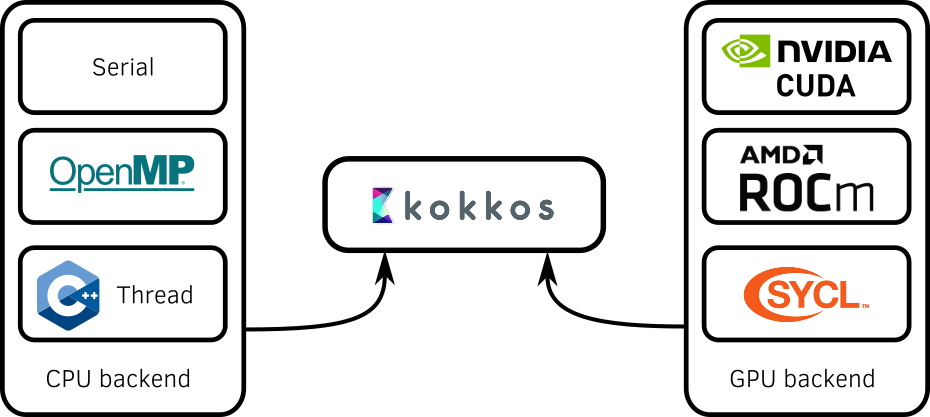
\includegraphics[width=0.6\textwidth]{kokkos_backend.png}
    \end{center}
\end{frame}

\begin{frame}[fragile]{Compiling Kokkos with the default parameters}
    \begin{columns}
        \begin{column}{0.6\linewidth}
            \begin{itemize}
                \item Defaults to the serial backend
                \item Use the default compiler or specify it with \texttt{-DCMAKE\_CXX\_COMPILER=<command>}
                \item Minimum supported version of the compilers detailed \href{https://kokkos.org/kokkos-core-wiki/get-started/requirements.html}{in the doc}
            \end{itemize}

            \vspace{-0.5em}

            \begin{minted}{bash}
                cmake \
                    -B ${build_dir} \
                    -DCMAKE_BUILD_TYPE=Release \
                    -DCMAKE_CXX_COMPILER=g++
                cmake \
                    --build ${build_dir} \
                    --parallel ${jobs}
                cmake \
                    --install ${build_dir} \
                    --prefix ${path_to_kokkos}
            \end{minted}
        \end{column}
        \pause
        \begin{column}{0.4\linewidth}
            \begin{center}
                \small
                \begin{table}{Compilers}{lll}
                    Name       & Cmd.             & Min.\ ver. \\\hline
                    Clang      & \texttt{clang++} & 15.0.0     \\
                    GCC        & \texttt{g++}     & 10.4.0     \\
                    Intel LLVM & \texttt{icpx}    & 2024.2.1   \\
                    NVHPC      & \texttt{nvc++}   & 22.3       \\
                    ROCM       & \texttt{hipcc}   & 6.2.0
                \end{table}
            \end{center}
        \end{column}
    \end{columns}
\end{frame}

\begin{frame}{Compiling Kokkos for a specific CPU architecture}
    \begin{columns}
        \begin{column}{0.4\linewidth}
            \begin{itemize}
                \item Add the architecture option \texttt{-DKokkos\_ARCH\_<NAME>=ON}
                \item CPU architecture is optional, for optimization (and vectorization)
                \item All CMake options are available \href{https://kokkos.org/kokkos-core-wiki/get-started/configuration-guide.html}{in the doc}
            \end{itemize}
        \end{column}
        \pause
        \begin{column}{0.6\linewidth}
            \begin{center}
                \small
                \begin{table}{CPU architectures}{ll}
                    CPU model & Option \\\hline
                    & \texttt{-DKokkos\_ARCH\_NATIVE=ON} \\
                    AMD Zen5 & \texttt{-DKokkos\_ARCH\_ZEN5=ON} \\
                    Intel Icelake & \texttt{-DKokkos\_ARCH\_ICX=ON} \\
                    NVIDIA Grace & \texttt{-DKokkos\_ARCH\_ARMV9\_GRACE=ON} \\
                \end{table}
            \end{center}
        \end{column}
    \end{columns}
\end{frame}

\begin{frame}{How to add Kokkos to your project}
    \begin{itemize}
        \item Kokkos only uses CMake (no Makefiles!)
        \item There are several ways to do it (for lack of a standard C++ dependency manager)
        \begin{itemize}
            \item Build and install it
            \item As a Git submodule
            \item Using CMake FetchContent
            \item With Spack
        \end{itemize}
        \item None of them is the perfect solution
    \end{itemize}
\end{frame}

\begin{frame}{Different ways to handle the Kokkos dependency}
    \begin{columns}[T]
        \begin{column}{0.25\linewidth}
            \strut Build and install

            \emph{\small\strut(external library)}

            \begin{block}{Pros}
                \begin{itemize}
                    \item You build Kokkos once
                \end{itemize}
            \end{block}
            \begin{alertblock}{Cons}
                \begin{itemize}
                    \item Not flexible
                    \item Not dev-friendly
                    \item Dependency up to the user
                \end{itemize}
            \end{alertblock}
        \end{column}
        \pause
        \begin{column}{0.25\linewidth}
            \strut Git submodule

            \emph{\small\strut(inline build)}

            \begin{block}{Pros}
                \begin{itemize}
                    \item Easy
                    \item Popular
                \end{itemize}
            \end{block}
            \begin{alertblock}{Cons}
                \begin{itemize}
                    \item User may forget to get the submodule
                    \item Not very clean
                \end{itemize}
            \end{alertblock}
        \end{column}
        \pause
        \begin{column}{0.25\linewidth}
            \strut CMake FetchContent

            \emph{\small\strut(inline build)}

            \begin{block}{Pros}
                \begin{itemize}
                    \item Trivial for the user
                \end{itemize}
            \end{block}
            \begin{alertblock}{Cons}
                \begin{itemize}
                    \item Not trivial for the dev to do it right
                    \item Not very clean
                \end{itemize}
            \end{alertblock}
        \end{column}
        \pause
        \begin{column}{0.25\linewidth}
            \strut Spack

            \emph{\small\strut(external library)}

            \begin{block}{Pros}
                \begin{itemize}
                    \item Good for production
                    \item Has dev mode
                    \item Can bring the backend libs
                \end{itemize}
            \end{block}
            \begin{alertblock}{Cons}
                \begin{itemize}
                    \item Not trivial
                \end{itemize}
            \end{alertblock}
        \end{column}
    \end{columns}
\end{frame}

\begin{exerciseframe}{Build Kokkos for the Serial backend}
    \begin{columns}
        \begin{column}{0.55\linewidth}
            \begin{minted}[breakafter={=}]{sh}
                cmake \
                    -S /src/kokkos \
                    -B build/serial \
                    -DCMAKE_BUILD_TYPE=Release

                cmake \
                    --build build/serial \
                    --parallel 4

                cmake \
                    --install build/serial \
                    --prefix $HOME/opt/kokkos/serial
            \end{minted}
        \end{column}
        \begin{column}{0.45\linewidth}
            \begin{itemize}
                \item Build and install Kokkos with the Serial backend
            \end{itemize}
        \end{column}
    \end{columns}
\end{exerciseframe}

\section{First steps with Kokkos}

\begin{frame}[fragile]{Start a Kokkos program}
    \begin{columns}
        \begin{column}{0.6\linewidth}
            \begin{minted}{C++}
                #include <Kokkos_Core.hpp>

                int main(int argc, char* argv[]) {
                    Kokkos::initialize(argc, argv);
                    {
                        // Your code here
                    }
                    Kokkos::finalize();
                }
            \end{minted}
        \end{column}
        \begin{column}{0.4\linewidth}
            \begin{itemize}
                \item Include the Kokkos header file (like any other library)
                \item Use the Kokkos namespace \texttt{Kokkos::}
                \item Initialize and finalize Kokkos (like MPI)
            \end{itemize}
        \end{column}
    \end{columns}
\end{frame}

\begin{frame}[fragile]{Start a Kokkos program (RAII)}
    \begin{columns}
        \begin{column}{0.6\linewidth}
            \begin{minted}{C++}
                #include <Kokkos_Core.hpp>

                int main(int argc, char* argv[]) {
                    Kokkos::ScopeGuard guard(argc, argv);

                    // Your code here
                }
            \end{minted}
        \end{column}
        \begin{column}{0.4\linewidth}
            \begin{itemize}
                \item \texttt{ScopeGuard} is a class that ensures that \texttt{Kokkos::initialize} and \texttt{Kokkos::finalize} are called correctly
                \item Resource Acquisition Is Initialization (RAII) pattern
            \end{itemize}
        \end{column}
    \end{columns}
\end{frame}

\begin{frame}[fragile]{Hello world}
    \begin{columns}
        \begin{column}{0.6\linewidth}
            \begin{minted}{C++}
                Kokkos::printf("Hello %s!\n", "world");
            \end{minted}
        \end{column}
        \begin{column}{0.4\linewidth}
            \begin{itemize}
                \item \texttt{printf} function to print things (works like \texttt{std::print} of C++23, with the syntax of \texttt{std::printf})
                \item Works anywhere (even on GPU)!
            \end{itemize}
        \end{column}
    \end{columns}
\end{frame}

\begin{frame}[fragile]{Use CMake to compile your Kokkos program}
    \begin{columns}
        \begin{column}{0.6\linewidth}
            \begin{minted}{cmake}
                cmake_minimum_required(VERSION 3.22)

                project(my_kokkos_project LANGUAGES CXX)

                find_package(Kokkos REQUIRED)

                add_executable(proj main.cpp)
                target_link_libraries(proj Kokkos::kokkos)
            \end{minted}
        \end{column}
        \begin{column}{0.4\linewidth}
            \begin{itemize}
                \item \texttt{find\_package} command to find Kokkos
                \item \texttt{REQUIRED} aborts the configuration if Kokkos is not found
                \item \texttt{target\_link\_libraries} command to link your program with Kokkos
                \item This is the "Kokkos is built and installed" and "Spack" approaches
            \end{itemize}
        \end{column}
    \end{columns}
\end{frame}

\begin{frame}[fragile]{Build your Kokkos program}
    \begin{columns}
        \begin{column}{0.6\linewidth}
            \begin{minted}{bash}
                # configure
                cmake \
                    -B ${build_dir} \
                    -DCMAKE_CXX_COMPILER=${compiler} \
                    -DKokkos_ROOT=${path_to_kokkos} \
                    ${other_options}

                # build
                cmake \
                    --build ${build_dir} \
                    --parallel ${jobs}
            \end{minted}
        \end{column}
        \begin{column}{0.4\linewidth}
            \begin{itemize}
                \item Kokkos propagates its compilation flags to your program
                \item \texttt{-DKokkos\_ROOT} to tell where Kokkos is installed
                \item You may want to add \texttt{-DCMAKE\_BUILD\_TYPE=<Mode>}
                \item Build in parallel
            \end{itemize}
        \end{column}
    \end{columns}
\end{frame}

\begin{exerciseframe}{From the "hello\_world" folder}
    \begin{columns}
        \begin{column}{0.5\linewidth}
            \begin{minted}[breakafter={=}]{sh}
                cmake \
                    -B build/serial \
                    -DCMAKE_BUILD_TYPE=Release \
                    -DKokkos_ROOT=$HOME/opt/kokkos/serial

                cmake \
                    --build build/serial
            \end{minted}
        \end{column}
        \begin{column}{0.5\linewidth}
            \begin{itemize}
                \item Build the hello world code
                \item Run with the \texttt{--kokkos-print-configuration} argument
            \end{itemize}
        \end{column}
    \end{columns}
\end{exerciseframe}

\section{Sequential implementation of the Gray--Scott equation}

\begin{exerciseframe}{From the "sequential" folder}
    \begin{columns}
        \begin{column}{0.5\linewidth}
            \begin{minted}[breakafter={=}]{sh}
                cmake \
                    -B build/serial \
                    -DCMAKE_BUILD_TYPE=Release

                cmake \
                    --build build/serial
            \end{minted}
        \end{column}
        \begin{column}{0.5\linewidth}
            \begin{itemize}
                \item Check the implementation
                \item Build the code
                \item No need for Kokkos here
                \item Run it
            \end{itemize}
        \end{column}
    \end{columns}
\end{exerciseframe}

\section{Data containers}

\begin{frame}[fragile]{Kokkos' abstracted data container}
    \begin{itemize}
        \item Why is it important to have an abstracted data container?
        \begin{itemize}
            \item<1-> No need to allocate or deallocate memory by hand
            \item<2-> Unified semantic and portable memory management (CPU and GPU)
            \item<3-> Vendor-specific memory allocation is hidden
            \item<4-> Advanced capabilities (abstracted layout, subarray, multidimensionality, etc.)
            \item<5-> Safety, through runtime or compile time checks
        \end{itemize}
        \item<6-> Kokkos provides the View class
        \begin{itemize}
            \item<7-> View is an abstraction of the notion of container and multidimensional array
            \item<8-> Brings portable Python numpy/Fortran-like syntax
        \end{itemize}
    \end{itemize}
\end{frame}

\begin{frame}[fragile]{Creating a View}
    \begin{columns}
        \begin{column}{0.6\linewidth}
            \begin{minted}{C++}
                Kokkos::View<float*>
                    view1("dynamic size", 10);

                Kokkos::View<int[100]>
                    view2("static size");

                Kokkos::View<double*[10]>
                    view3("static and dynamic size", 10);

                Kokkos::View<double***[10]>
                    view4("four dimensions", 10, 10, 10);
            \end{minted}
        \end{column}
        \begin{column}{0.4\linewidth}
            \begin{itemize}
                \item View is a template class
                \item Contains any C++ type (\texttt{int}, \texttt{float}, \texttt{double}, etc)
                \item Number of dimensions, fixed at compile time (no more than 7)
                \item Size of each dimension determined at...
                \begin{description}[\texttt{[n]}]
                    \item[\texttt{*}] runtime
                    \item[\texttt{[n]}] compile time
                \end{description}
            \end{itemize}
        \end{column}
    \end{columns}
\end{frame}

\begin{frame}[fragile]{Creating a View (2)}
    \begin{columns}
        \begin{column}{0.6\linewidth}
            \begin{minted}{C++}
                Kokkos::View<float*>
                    view1("dynamic size", 10);

                Kokkos::View<int[100]>
                    view2("static size");

                Kokkos::View<double*[10]>
                    view3("static and dynamic size", 10);

                Kokkos::View<double***[10]>
                    view4("four dimensions", 10, 10, 10);
            \end{minted}
        \end{column}
        \begin{column}{0.4\linewidth}
            \begin{itemize}
                \item Name (useful for debugging!)
                \item Check at compile time and runtime (out of bound, same size for operations, ...)
            \end{itemize}
        \end{column}
    \end{columns}
\end{frame}

\begin{frame}[fragile]{Accessing the data}
    \begin{columns}
        \begin{column}{0.6\linewidth}
            \begin{minted}{C++}
                const int Nx = 1000;
                const int Ny = 2000;

                Kokkos::View<int**>
                    my_matrix("matrix", Nx, Ny);

                for (int i = 0; i < Nx; i++) {
                    for (int j = 0; j < Ny; j++) {
                        my_matrix(i, j) = i + j;
                    }
                }
            \end{minted}
        \end{column}
        \begin{column}{0.4\linewidth}
            \begin{itemize}
                \item Data are accessed using the parenthesis operator \texttt{(i, j, k, ...)}
                \item Raw data can be accessed using the \texttt{data()} method (not recommended)
            \end{itemize}
        \end{column}
    \end{columns}
\end{frame}

\begin{frame}[fragile]{Basic methods to manage views}
    \begin{columns}
        \begin{column}{0.45\linewidth}
            \begin{minted}{C++}
                Kokkos::View<int ***>
                    view("view", 10, 20, 30);

                int rank = view.rank();
                assert(rank == 3);

                int size_x = view.extent(0);
                assert(size_x == 10);

                int size = view.size();
                assert(size == 6000);
            \end{minted}
        \end{column}
        \begin{column}{0.55\linewidth}
            \begin{description}[\texttt{extent(dim)}]
                \item[\texttt{rank()}] Return the rank of the view (number of dimensions)
                \item[\texttt{extent(dim)}] Return the number of elements of a specific dimension
                \item[\texttt{size()}] Return the total number of elements
            \end{description}

            \vspace{0.5em}

            And many others not covered in this talk
        \end{column}
    \end{columns}
\end{frame}

\begin{frame}{Notion of View layout}
    \begin{center}
        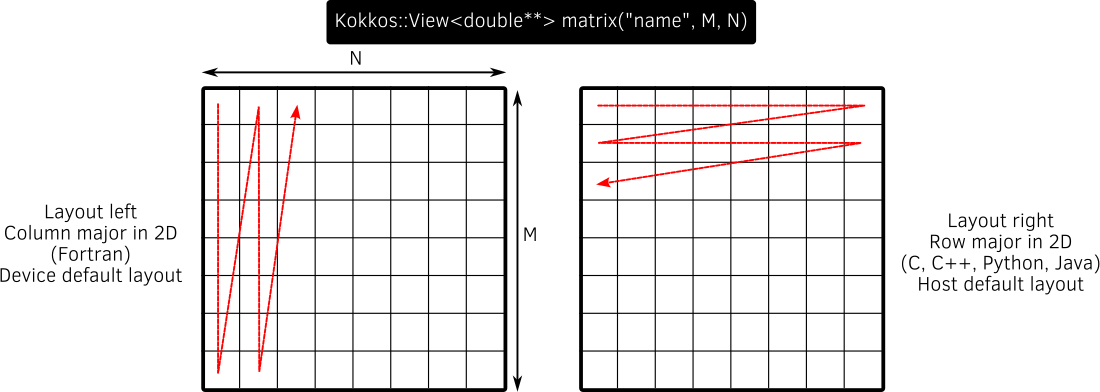
\includegraphics[width=0.8\textwidth]{layout_right_left.png}
    \end{center}
    \begin{itemize}
        \item Layout is the way multidimensional indices map to linear memory
        \item Kokkos provides an abstraction of the data layout
        \item The default layout of a View depends on the backend (Host or Device)
    \end{itemize}
\end{frame}

\begin{frame}[fragile]{How to set a View layout}
    \begin{columns}
        \begin{column}{0.5\linewidth}
            \begin{minted}{C++}
                Kokkos::View<int**, Layout>
                    my_matrix("matrix", 10, 10);
            \end{minted}
        \end{column}
        \begin{column}{0.5\linewidth}
            \begin{itemize}
                \item Template argument \texttt{Layout} to specify the layout when creating a view
                \item Several ones available (Left, Right, Stride, ...)
                \item Possible to define your own custom layout
                \item Default values are usually sufficient for basic usages
            \end{itemize}
        \end{column}
    \end{columns}
\end{frame}

\begin{frame}{More about views}
    \begin{itemize}
        \item Allocations only happen when explicitly specified
        \pause
        \item Reference counting is used for automatic deallocation (like shared pointers)
        \pause
        \item Copy construction and assignment are shallow: you pass Views by value, not by pointer (e.g. C arrays); you can still pass by constant reference
    \end{itemize}
\end{frame}

\begin{frame}[fragile]{Copy and assignation}
    \begin{columns}
        \begin{column}{0.65\linewidth}
            \begin{minted}{C++}
                Kokkos::View<int*[5]> a("a", 10), b("b", 15);
                a = b;
                Kokkos::View<int**> c(b);

                a(0, 2) = 1;
                b(0, 2) = 2;
                c(0, 2) = 3;

                std::cout << a(0, 2) << std::endl;
            \end{minted}
        \end{column}
        \begin{column}{0.35\linewidth}
            \begin{block}{What gets printed?}
                \pause
                3
            \end{block}
        \end{column}
    \end{columns}
\end{frame}

\begin{exerciseframe}{From the "sequential" folder}
    \begin{columns}
        \begin{column}{0.5\linewidth}
            \begin{minted}{C++}
                #include <Kokkos_Core.hpp>

                // ...

                using View =
                    Kokkos::View<double **>;

                View a("A", N, M);
                a(0, 1) = 1;
            \end{minted}
        \end{column}
        \begin{column}{0.5\linewidth}
            \begin{itemize}
                \item Duplicate the \texttt{sequential} folder to a different name
                \item Add the Kokkos header
                \item Use Kokkos views instead of plain-old-data arrays for \texttt{u} and \texttt{v} (and temporary arrays) in \texttt{main} and in \texttt{compute}
                \item For now, just pass a raw pointer when calling \texttt{check} and \texttt{print\_field}
                \item The checksum must remain the same!
            \end{itemize}
        \end{column}
    \end{columns}
\end{exerciseframe}


\begin{frame}{Subviews description (bonus)}
    \begin{itemize}
        \item A subview is a ’slice’ of a View that behaves as a View
        \pause
        \begin{itemize}
            \item Same syntax as a View - access data using (multi-)index entries
            \pause
            \item The ’slice’ and original View point to the same data - no extra
            memory allocation or copying
        \end{itemize}
        \pause
        \item Can be constructed on host or within a kernel (no allocation
        of memory occurs)
        \pause
        \item Similar capability as provided by Matlab, Fortran, Python, etc.
        using ’colon’ notation
    \end{itemize}
\end{frame}

\begin{frame}[fragile]{Usage demo}
    Begin with a View:
    \begin{minted}{C++}
        Kokkos::View<double ***> v("v", N0, N1, N2);
    \end{minted}
    \pause
    Say we want a 2-dimensional slice at an index i0 in the first
    dimension - that is, in Matlab/Fortran/Python notation:
    \begin{minted}{python}
        slicei0 = v[i0, :, :]
    \end{minted}
    \pause
    This can be accomplished in Kokkos using a subview as follows:
    \begin{minted}{C++}
        auto slice = Kokkos::subview(v, i0, Kokkos::ALL, Kokkos::ALL);
    \end{minted}
\end{frame}

\begin{frame}[fragile]{Syntax}
    \begin{minted}{C++}
        Kokkos::subview(view, arg0, ...);
    \end{minted}
    \begin{itemize}
        \item \texttt{view}: First argument to the subview is the view of which a slice will be taken
        \item \texttt{argN}: Slice info for rank $N$ - provide same number of arguments as rank
        \item Options for \texttt{argN}:
        \begin{description}[partial range]
            \item[index] integral type single value
            \item[partial range] \texttt{std::pair} or \texttt{Kokkos::pair} of integral types to provide sub-range of a rank’s range $[0, N)$
            \item[full range] use \texttt{Kokkos::ALL} rather than providing the full range as a pair
        \end{description}
    \end{itemize}
\end{frame}

\begin{frame}[fragile]{Subviews suggested usage}
    \begin{itemize}
        \item Use \texttt{auto} to determine the return type of a subview
        \item A subview can help with encapsulation - e.g. can pass into functions expecting a lower-dimensional View
        \item Use \texttt{Kokkos::pair} for partial ranges if subview created within a kernel
        \item Avoid usage if very few data accesses will be made to the subview
        \begin{itemize}
            \item Construction of subview costs 20-40 operations
        \end{itemize}
    \end{itemize}
\end{frame}

\section{Parallel loops}

\begin{frame}[fragile]{Anatomy of a loop}
    \begin{columns}
        \begin{column}{0.5\linewidth}
            \begin{minted}[texcomments]{C++}
                for (int i = 0; i < N; i++) {
                    A(i) = B(i) + C(i) * D(i);
                }
            \end{minted}
        \end{column}
        \begin{column}{0.5\linewidth}
            \begin{itemize}
                \item \mintinline{C++}{for} is the loop pattern (for, reduction, scan, graph)
                \item \mintinline{C++}{int i = 0; i < N; i++} is the execution policy
                \item \mintinline{C++}{A(i) = B(i) + C(i) * D(i)} is the kernel
                \begin{itemize}
                    \item No iteration order dependencies
                    \item No side effects
                \end{itemize}
            \end{itemize}
        \end{column}
    \end{columns}
\end{frame}

\begin{frame}[fragile]{Comparison of Kokkos and OpenMP parallel loops}
    \begin{columns}[T]
        \begin{column}{0.5\linewidth}
            \begin{center}
                \textbf{OpenMP version}
            \end{center}
            \begin{minted}{C++}
                #pragma omp parallel for
                for (int i = 0; i < N; i++) {
                    A(i) = B(i) + C(i) * D(i);
                }
            \end{minted}
            \begin{block}{Note}
                Only works on CPUs (needs the \texttt{target} directive for GPUs)
            \end{block}
        \end{column}
        \pause
        \begin{column}{0.5\linewidth}
            \begin{center}
                \textbf{Kokkos version}
            \end{center}
            \begin{minted}{C++}
                Kokkos::parallel_for(
                    "my_loop",
                    N,
                    KOKKOS_LAMBDA (int i) {
                        A(i) = B(i) + C(i) * D(i);
                    }
                );
            \end{minted}

            \vspace{-0.75em}

            \begin{block}{Note}
                Works on CPUs and GPUs depending on the compiled backend
            \end{block}
        \end{column}
    \end{columns}
\end{frame}

\begin{frame}[fragile]{Anatomy of a Kokkos parallel loop}
    \begin{columns}
        \begin{column}{0.5\linewidth}
            \begin{minted}{C++}
                Kokkos::parallel_for(
                    "my_loop",
                    N,
                    KOKKOS_LAMBDA (int i) {
                        A(i) = B(i) + C(i) * D(i);
                    }
                );
            \end{minted}
        \end{column}
        \begin{column}{0.5\linewidth}
            \begin{itemize}
                \item \mintinline{C++}{parallel_for} is the loop pattern
                \item \mintinline{C++}{"my_loop"} is the name of the loop (bonus for debugging!)
                \item \mintinline{C++}{N} and \mintinline{C++}{int i} is the execution policy (can't be simpler)
                \item \mintinline[breaklines]{C++}{KOKKOS_LAMBDA (int i) {/*...*/}} is the kernel
            \end{itemize}
        \end{column}
    \end{columns}

    \pause

    \begin{block}{Question}
         What is this \texttt{KOKKOS\_LAMBDA} thingy?
    \end{block}
\end{frame}

\begin{frame}[fragile]{Notion of C++ lambdas}
    \begin{columns}
        \begin{column}{0.5\linewidth}
            \begin{minted}{C++}
                auto kernel =
                    KOKKOS_LAMBDA (int i) {
                        A(i) = B(i) + C(i) * D(i);
                    };
            \end{minted}
        \end{column}
        \begin{column}{0.5\linewidth}
            \begin{itemize}
                \item A lambda is a C++ anonymous function (i.e. a function as an object)
                \item It has explicit arguments (\mintinline{C++}|int i|) and captured objects (\mintinline{C++}|A|, \mintinline{C++}|B|, \mintinline{C++}|C|, \mintinline{C++}|D|)
                \item \texttt{KOKKOS\_LAMBDA} is a macro that creates a lambda function with the correct capture for you (and a bit more)
                \item We will give more details about it next week
            \end{itemize}
        \end{column}
    \end{columns}
\end{frame}

\begin{frame}[fragile]{How to extend loop policies?}
    \begin{columns}
        \begin{column}{0.55\linewidth}
            \begin{minted}{C++}
                Kokkos::RangePolicy<ExecutionSpace>
                    policy(start_index, end_index);
            \end{minted}
        \end{column}
        \begin{column}{0.45\linewidth}
            \begin{itemize}
                \item Kokkos way to tell how a loop is executed: \structure{execution policy}
                \item \mintinline{c++}|RangePolicy| for single-dimensional loops
                \item \mintinline{c++}|ExecutionSpace| for specifying where the loop is executed (we'll discuss about this next week, you can keep the default value for now)
                \item \mintinline{c++}|start_index| and \mintinline{c++}|end_index| are the beginning (inclusive) and the end (exclusive) of the loop
            \end{itemize}
        \end{column}
    \end{columns}
\end{frame}

\begin{frame}[fragile]{Loop policy shortcut}
    \begin{columns}
        \begin{column}{0.45\linewidth}
            Shortcut version\strut

            \begin{minted}{C++}
                Kokkos::parallel_for(
                    "my_loop",
                    N,
                    KOKKOS_LAMBDA (int i) {
                        /* ... */
                    }
                );
            \end{minted}
        \end{column}
        \pause
        \begin{column}{0.55\linewidth}
            Explicit version (same)\strut

            \begin{minted}{C++}
                Kokkos::parallel_for(
                    "my_loop",
                    Kokkos::RangePolicy<>(0, N),
                    KOKKOS_LAMBDA (int i) {
                        /* ... */
                    }
                );
            \end{minted}
        \end{column}
    \end{columns}
\end{frame}

\begin{frame}[fragile]{Anatomy of a nested loops}
    \begin{columns}
        \begin{column}{0.5\linewidth}
            \begin{minted}{C++}
                for (int i = 0; i < Nx; i++)
                    for (int j = 0; j < Ny; j++) {
                        A(i, j) = i + j;
                    }
            \end{minted}
        \end{column}
        \begin{column}{0.5\linewidth}
            \begin{itemize}
                \item 2 loop patterns
                \begin{itemize}
                    \item No extra code before/after the inner loop
                    \item Loops are collapsible (OpenMP \texttt{collapse})
                \end{itemize}
                \item 2 execution policies
                \begin{itemize}
                    \item No dependencies between them
                \end{itemize}
                \item 1 kernel
                \begin{itemize}
                    \item No iteration order dependencies
                    \item No side effects
                \end{itemize}
            \end{itemize}
        \end{column}
    \end{columns}
\end{frame}

\begin{frame}[fragile]{How to have multidimensional loop policies?}
    \begin{columns}
        \begin{column}{0.66\linewidth}
            \begin{minted}{C++}
                Kokkos::MDRangePolicy<
                    Kokkos::Rank<N>
                > policy(
                    {start_index_0, /* ... */, start_index_n},
                    {end_index_0, /* ... */, end_index_n}
                );
            \end{minted}
        \end{column}
        \begin{column}{0.34\linewidth}
            \begin{itemize}
                \item \mintinline{C++}|MDRangePolicy| for nested loops (with \emph{MD} for multidimensional)
                \item \mintinline{C++}|Rank| template parameter to specify the dimension
                \item Max rank is 6
                \item \mintinline{C++}|start_index_*| and \mintinline{C++}|end_index_*| are the beginning (inclusive) and the end (exclusive) of each loop
            \end{itemize}
        \end{column}
    \end{columns}
\end{frame}

\begin{frame}[fragile]{Anatomy of a Kokkos nested loop}
    \begin{columns}
        \begin{column}{0.6\linewidth}
            \begin{minted}{C++}
                Kokkos::parallel_for(
                    "my_loop",
                    Kokkos::MDRangePolicy<
                        Kokkos::Rank<2>
                    >(
                        {0, 0},
                        {Nx, Ny}
                    ),
                    KOKKOS_LAMBDA (int i, int j) {
                        A(i, j) = i + j;
                    }
                );
            \end{minted}
        \end{column}
        \begin{column}{0.4\linewidth}
            \begin{itemize}
                \item Still 1 \texttt{parallel\_for}
                \item No shortcut version!
                \item Kernel has 2 arguments
            \end{itemize}
        \end{column}
    \end{columns}
\end{frame}

\begin{exerciseframe}{From your worktree}
    \begin{columns}
        \begin{column}{0.5\linewidth}
            \begin{minted}{C++}
                Kokkos::parallel_for(
                    "my_loop",
                    Kokkos::MDRangePolicy<
                        Kokkos::Rank<2>
                    >(
                        {0, 0},
                        {Nx, Ny}
                    ),
                    KOKKOS_LAMBDA (int i, int j) {
                        A(i, j) = i + j;
                    }
                );
            \end{minted}
        \end{column}
        \begin{column}{0.5\linewidth}
            \begin{itemize}
                \item Use Kokkos \texttt{parallel\_for} and \texttt{MDRangePolicy} instead of the nested loops in \texttt{compute} (additionally in \texttt{add\_drop})
                \item The checksum must remain the same!
            \end{itemize}
        \end{column}
    \end{columns}
\end{exerciseframe}

\section{Parallel reductions}

\begin{frame}[fragile]{Anatomy of a reduction loop}
    \begin{columns}
        \begin{column}{0.5\linewidth}
            \begin{minted}[texcomments]{C++}
                double result = 0;

                for (int i = 0; i < N; i++) {
                    result += A(i);
                }
            \end{minted}
        \end{column}
        \begin{column}{0.5\linewidth}
            \begin{itemize}
                \item One scalar variable collects something for each iteration (sum, max, min, etc.), to produce one final global result
                \pause
                \item Horrible truth: \mintinline{c++}{result} could \structure{depend} on iteration order!
                \item This is due to floating point arithmetic not being associative and to unknown iteration order
            \end{itemize}
        \end{column}
    \end{columns}
\end{frame}

\begin{frame}[fragile]{Anatomy of a Kokkos parallel reduction loop}
    \begin{columns}
        \begin{column}{0.5\linewidth}
            \begin{minted}{C++}
                // no initialization needed,
                // handled by parallel_reduce
                double result;

                Kokkos::parallel_reduce(
                    "my_reduction",
                    N,
                    KOKKOS_LAMBDA (
                        const int i,
                        double& local_result
                    ) {
                        local_result += i;
                    },
                    Kokkos::Sum<double>(result)
                );
            \end{minted}
        \end{column}
        \begin{column}{0.5\linewidth}
            \begin{itemize}
                \item \mintinline{c++}{parallel_reduce} to perform reductions
                \item Works like \texttt{parallel\_for} (e.g. execution policy, etc.)
                \item Reducer object (here \mintinline{c++}{Sum}), templated with the result type
                \item Extra last argument to the kernel: a reference to the local result
                \item Update local result in a manner consistent with global result
                \item The local result is write-only (it's a partial result)
            \end{itemize}
        \end{column}
    \end{columns}
\end{frame}

\begin{frame}{About reducers}
    \begin{itemize}
        \item Kokkos provides implementations of Reducer classes for the most common operations:
        \begin{itemize}
            \item \texttt{Kokkos::Sum}: Sum of the elements
            \item \texttt{Kokkos::Max}: and \texttt{Kokkos::Min}: Maximum and minimum element
            \item \texttt{Kokkos::Prod}: Product of the elements
            \item \texttt{Kokkos::MaxLoc} and \texttt{Kokkos::MinLoc}: Maximum and minimum element with their index
            \item More \href{https://kokkos.org/kokkos-core-wiki/ProgrammingGuide/Custom-Reductions-Built-In-Reducers.html}{in the doc}
        \end{itemize}
        \item You can also create your own Reducer class, not covered in this talk
    \end{itemize}
\end{frame}

\begin{frame}[fragile]{Sum reduction example}
    \begin{minted}[fontsize=\scriptsize]{C++}
        double result;
        Kokkos::View<double*> A;
        ...
        Kokkos::parallel_reduce(
            "my_reduction",
            N,
            KOKKOS_LAMBDA (const int i, double& local_result) {
                local_result += A(i);
            },
            result // Only in the case of Sum, no need of the Reducer object
        );
    \end{minted}
\end{frame}

\begin{frame}[fragile]{Max reduction example}
    \begin{minted}[fontsize=\scriptsize]{C++}
        double max_value;
        Kokkos::View<double*> A;
        ...
        Kokkos::parallel_reduce(
            "my_reduction",
            N,
            KOKKOS_LAMBDA (const int i, double& local_max_value) {
                local_max_value = Kokkos::max(A(i), local_max_value);
                // local reduction consistent with the Reducer object
            },
            Kokkos::Max<double>(max_value)
        );
    \end{minted}

    \pause

    \vspace{-1em}

    \begin{columns}[T]
        \begin{column}{0.41\linewidth}
            \begin{block}{Math operators}
                Notice that mathematical operators are in the \texttt{Kokkos} namespace
            \end{block}
        \end{column}
        \pause
        \begin{column}{0.59\linewidth}
            \begin{block}{Beware}
                \texttt{Kokkos::max} is a mathematical operator, \texttt{Kokkos::Max<double>} defines a Reducer object
            \end{block}
        \end{column}
    \end{columns}
\end{frame}

\begin{frame}[fragile]{Min and index reduction example}
    \begin{columns}
        \begin{column}{0.55\linewidth}
            \begin{minted}[fontsize=\scriptsize]{C++}
                    using minloc_type =
                        Kokkos::MinLoc<double, int>::value_type;

                    minloc_type minloc;
                    Kokkos::parallel_reduce(
                        "min_loc_reduction",
                        N,
                        KOKKOS_LAMBDA (
                            int i,
                            minloc_type& local_minloc_value
                        ) {
                            if (A(i) < local_minloc_value.val) {
                                local_minloc_value.val = A(i);
                                local_minloc_value.loc = i;
                            }
                        },
                        Kokkos::MinLoc<double, int>(minloc)
                    );
                \end{minted}
        \end{column}
        \begin{column}{0.45\linewidth}
            \begin{itemize}
                \item Pay attention to the type of the intermediate and the global results
                \item Here, \texttt{Kokkos::MinLoc<double, int>::value\_type}: contains the value and the location
                \item In general, the type can be obtained as \texttt{value\_type} of the Reducer object
            \end{itemize}
        \end{column}
    \end{columns}
\end{frame}

\begin{frame}[fragile]{Combining multiple reductions}
    \begin{itemize}
        \item Multiple Reducer objects can be specified in the same \texttt{parallel\_reduce}
    \end{itemize}
    \begin{minted}[fontsize=\scriptsize]{C++}
        double sum_val,  min_val;

        Kokkos::parallel_reduce(
            "SumMinReduce", N,
            KOKKOS_LAMBDA (const int i, double& local_sum, double& local_min) {
                local_sum += A(i);
                local_min = Kokkos::min(A(i), local_min);
            },
            sum_val, Kokkos::Min<double>(min_val)
        );
    \end{minted}
\end{frame}

\begin{exerciseframe}{From your worktree}
    \begin{columns}
        \begin{column}{0.5\linewidth}
            \begin{minted}{C++}
                double result;
                Kokkos::parallel_reduce(
                    "my_reduction",
                    N,
                    KOKKOS_LAMBDA (
                        const int i,
                        double& local_result
                    ) {
                        local_result += A(i);
                    },
                    result
                );
            \end{minted}
        \end{column}
        \begin{column}{0.5\linewidth}
            \begin{itemize}
                \item Use Kokkos \texttt{parallel\_reduce} and \texttt{MDRangePolicy} instead of the nested loops in \texttt{check}
                \item The checksum must remain the same!
            \end{itemize}
        \end{column}
    \end{columns}
\end{exerciseframe}

\section{Moving to a parallel CPU backend}

\begin{exerciseframe}{(Re-)Initialization}
    \begin{columns}
        \begin{column}{0.6\linewidth}
            \begin{minted}[breakafter={/},fontsize=\scriptsize]{sh}
                srun ... --pty /bin/bash

                REPO=docker://gitlab-registry.in2p3.fr/thomas.padioleau/gray-scott-kokkos

                # pick one
                apptainer run $REPO/kokkos_cpu_interactive
                apptainer run $REPO/kokkos_cpu_interactive_jupyter
                apptainer run $REPO/kokkos_cpu_interactive_vscode
                apptainer run $REPO/kokkos_cpu_learning_platform_code_server

                cd $HOME/gray_scott_kokkos
            \end{minted}
        \end{column}
        \begin{column}{0.4\linewidth}
            \begin{itemize}
                \item Reserve a job for half a day (if needed, ask your satellite staff)
                \item Run Apptainer with the desired image
                \begin{itemize}
                    \item No editor
                    \item Jupyter
                    \item VSCode
                    \item CodeServer
                \end{itemize}
            \end{itemize}
        \end{column}
    \end{columns}
\end{exerciseframe}

\begin{frame}{The notion of backend in Kokkos}
    \begin{itemize}
        \item Kokkos is compiled to target a specific backend
        \item Kokkos is portable until you compile it
        \item You need one compilation per backend
    \end{itemize}
    \begin{center}
        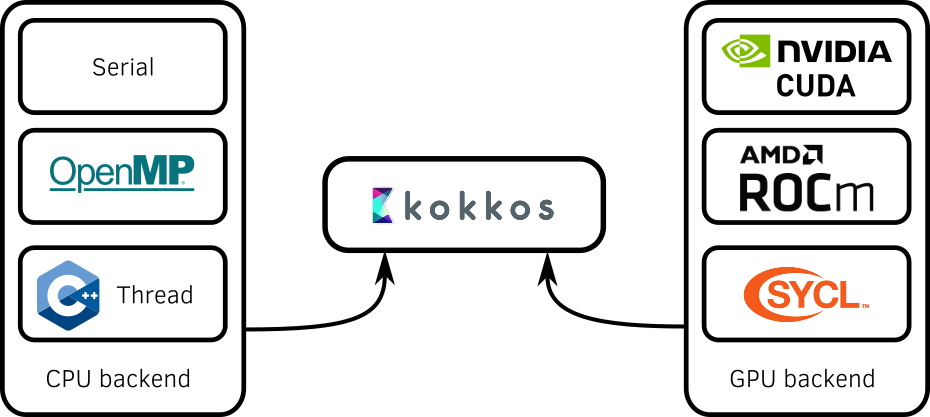
\includegraphics[width=0.6\textwidth]{kokkos_backend.png}
    \end{center}
\end{frame}

\begin{frame}[fragile]{Compiling Kokkos for a specific backend}
    \begin{columns}
        \begin{column}{0.46\linewidth}
            \begin{itemize}
                \item Add the option \texttt{-DKokkos\_ENABLE\_<BACKEND>=ON} to enable a specific backend
                \item Only one CPU backend can be compiled at a time (plus Serial backend)
            \end{itemize}
            \begin{minted}[texcomments]{bash}
                cmake \
                    -B ${build_dir} \
                    -DCMAKE_CXX_COMPILER=g++ \
                    -DKokkos_ENABLE_OPENMP=ON \
                    ${other_arguments}
            \end{minted}
        \end{column}
        \pause
        \begin{column}{0.54\linewidth}
            \begin{center}
                \begin{table}{CPU backends}{ll}
                    Backend & Option \\\hline
                    Serial & \texttt{-DKokkos\_ENABLE\_SERIAL=ON} \\
                    OpenMP & \texttt{-DKokkos\_ENABLE\_OPENMP=ON} \\
                    Threads & \texttt{-DKokkos\_ENABLE\_THREADS=ON}
                \end{table}
            \end{center}
        \end{column}
    \end{columns}
\end{frame}

\begin{exerciseframe}{Build Kokkos for the OpenMP backend}
    \begin{columns}
        \begin{column}{0.55\linewidth}
            \begin{minted}[breakafter={=}]{sh}
                cmake \
                    -S /src/kokkos \
                    -B build/openmp \
                    -DCMAKE_BUILD_TYPE=Release \
                    -DKokkos_ENABLE_OPENMP=ON \
                    -DKokkos_ARCH_NATIVE=ON

                cmake \
                --build build/openmp \
                --parallel 4

                cmake \
                --install build/openmp \
                --prefix $HOME/opt/kokkos/openmp
            \end{minted}
        \end{column}
        \begin{column}{0.45\linewidth}
            \begin{itemize}
                \item Build and install Kokkos with the OpenMP backend
                \item Pay attention to the \texttt{Kokkos\_ARCH\_NATIVE=ON} flag
            \end{itemize}
        \end{column}
    \end{columns}
\end{exerciseframe}

\begin{exerciseframe}{From the "hello\_world" folder}
    \begin{columns}
        \begin{column}{0.5\linewidth}
            \begin{minted}[breakafter={=}]{sh}
                cmake \
                    -B build/serial \
                    -DCMAKE_BUILD_TYPE=Release \
                    -DKokkos_ROOT=$HOME/opt/kokkos/openmp

                cmake \
                    --build build/openmp
            \end{minted}
        \end{column}
        \begin{column}{0.5\linewidth}
            \begin{itemize}
                \item Build the hello world code
                \item Run with the \texttt{--kokkos-print-configuration} argument
            \end{itemize}
        \end{column}
    \end{columns}
\end{exerciseframe}

\begin{exerciseframe}{From your worktree or the "cpu" folder}
    \begin{columns}
        \begin{column}{0.5\linewidth}
            \begin{minted}[breakafter={=}]{sh}
                cmake \
                -B build/openmp \
                -DCMAKE_BUILD_TYPE=Release \
                -DKokkos_ROOT=$HOME/opt/kokkos/openmp

                cmake \
                --build build/openmp
            \end{minted}
        \end{column}
        \begin{column}{0.45\linewidth}
            \begin{itemize}
                \item Build your code using this OpenMP instance of Kokkos
                \item Run with and without I/Os with the \texttt{time} command
            \end{itemize}
        \end{column}
    \end{columns}
\end{exerciseframe}

\section{Performance on CPU}

\begin{frame}[fragile]{Performance scaling in parallel computing}

\textbf{Scaling} describes how application performance changes as more compute
resources (CPU cores, nodes, GPUs) are added.

\vspace{0.5em}

\begin{center}
    \begin{table}{Two Fundamental Types}{l|ll}
        \textbf{Aspect} & \textbf{Strong Scaling} & \textbf{Weak Scaling} \\\hline
        Problem size & Fixed & Grows with processor count \\
        Work per processor & Decreases & Remains constant \\
        Goal & Reduce time-to-solution & \makecell[l]{Maintain runtime while solving\\larger problems} \\
    \end{table}
\end{center}

\begin{center}
\begin{tabular}{c|c|c}
\textbf{Processors} & \textbf{Strong Scaling} & \textbf{Weak Scaling} \\
\hline
1   & 1M points   & 1M points \\
10  & 1M points   & 10M points \\
\end{tabular}
\end{center}
\end{frame}

\begin{frame}[fragile]{Strong Scaling}

\begin{block}{Definition}
Strong scaling measures how execution time decreases when solving a
\textbf{fixed-size problem} using more processors
\end{block}

\begin{columns}
    \begin{column}{0.5\linewidth}
        \textbf{Ideal strong scaling}

        \[
        T(P) = \frac{T(1)}{P}
        \]

        \begin{itemize}
            \item $T(1)$: runtime on one thread
            \item $T(P)$: runtime on $P$ threads
        \end{itemize}

        \textbf{Strong scaling speedup}

        \[
        S(P) = \frac{T(1)}{T(P)}
        \]
    \end{column}
    \begin{column}{0.5\linewidth}
        \textbf{Common limitations}
        \begin{itemize}
            \item Communication overhead
            \item Synchronization costs
            \item Load imbalance
            \item Serial code sections (Amdahl's Law)
        \end{itemize}
    \end{column}
\end{columns}
\end{frame}

\begin{frame}[fragile]{Weak Scaling}

\begin{block}{Definition}
Weak scaling measures how runtime changes when \textbf{both the number of processors
and the total problem size} increase proportionally, keeping the workload per
processor approximately constant
\end{block}

\vspace{0.5em}

\begin{columns}
    \begin{column}{0.4\linewidth}
        \textbf{Ideal weak scaling}

        \[
        T(P) \approx T(1)
        \]

        \textbf{Weak scaling efficiency}

        \[
        E(P) = \frac{T(1)}{T(P)}
        \]
    \end{column}
    \begin{column}{0.6\linewidth}
        \textbf{Common limitations}
        \begin{itemize}
            \item Communication growth
            \item Network contention
            \item Collective operations (reductions, barriers)
            \item Memory and I/O bottlenecks
        \end{itemize}
    \end{column}
\end{columns}

\end{frame}

\begin{exerciseframe}{From your worktree or the "cpu" folder}
    \begin{itemize}
        \item Perform scalings
        \begin{itemize}
            \item Strong scaling
            \item Weak scaling
        \end{itemize}
        \item From 1 core to the maximum number of cores in the node
    \end{itemize}
\end{exerciseframe}

\begin{frame}{The Ruche supercomputer}
    \begin{description}[Location]
        \item[Name] Ruche cluster
        \item[Location] IDRIS, Moulon, Île-de-France
        \item[CPU] Intel Xeon Gold 6230, 2.1 GHz, 20 cores per socket, 2 sockets per node
    \end{description}
\end{frame}

\begin{frame}[fragile]{Example of weak scaling on Ruche}
    \begin{center}
        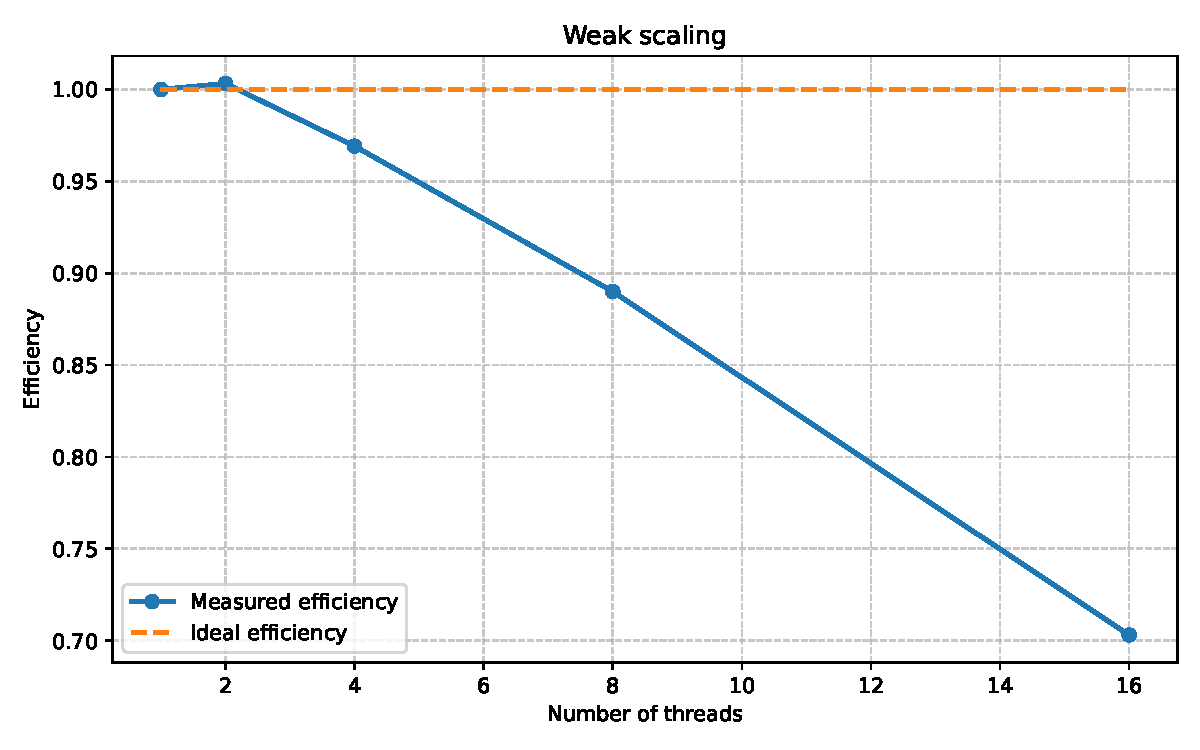
\includegraphics[width=0.8\textwidth]{weak_scaling_ruche.pdf}
    \end{center}
\end{frame}

\begin{frame}[fragile]{Example of strong scaling on Ruche}
    \begin{center}
        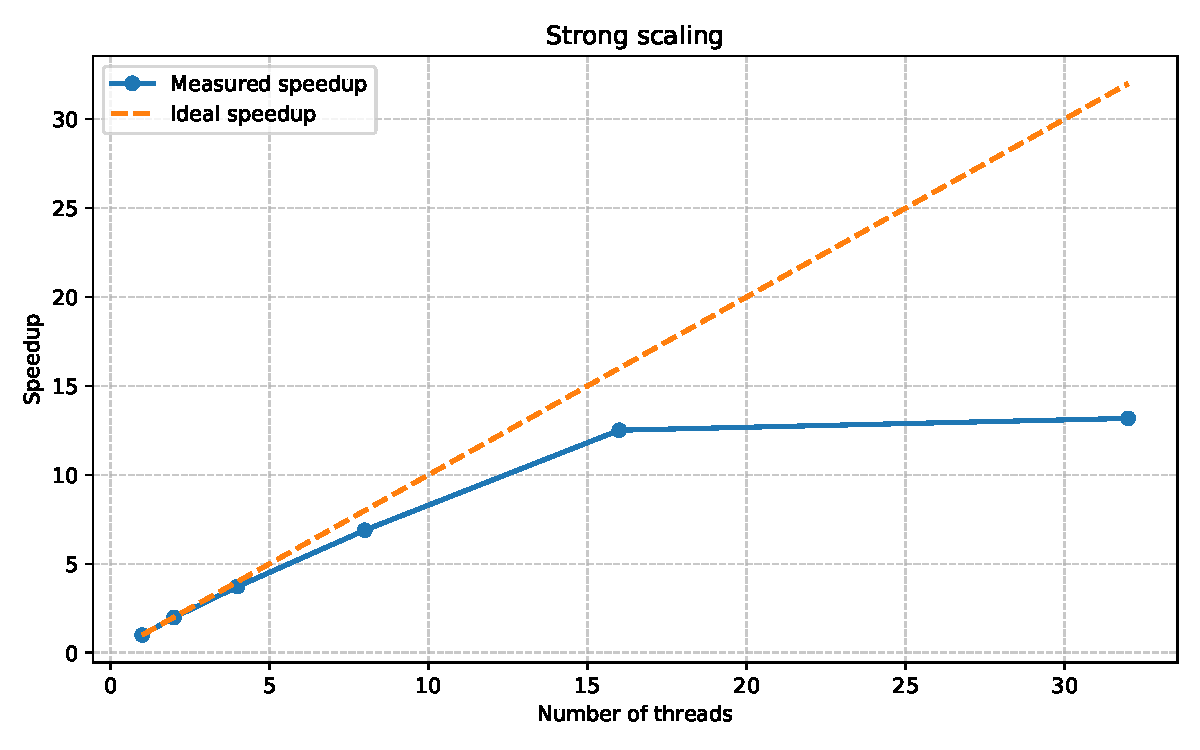
\includegraphics[width=0.8\textwidth]{strong_scaling_ruche.pdf}
    \end{center}
\end{frame}

\section{SIMD and vectorization}

\begin{frame}[fragile]{What is vectorization}
    \begin{columns}
        \begin{column}{0.5\linewidth}
            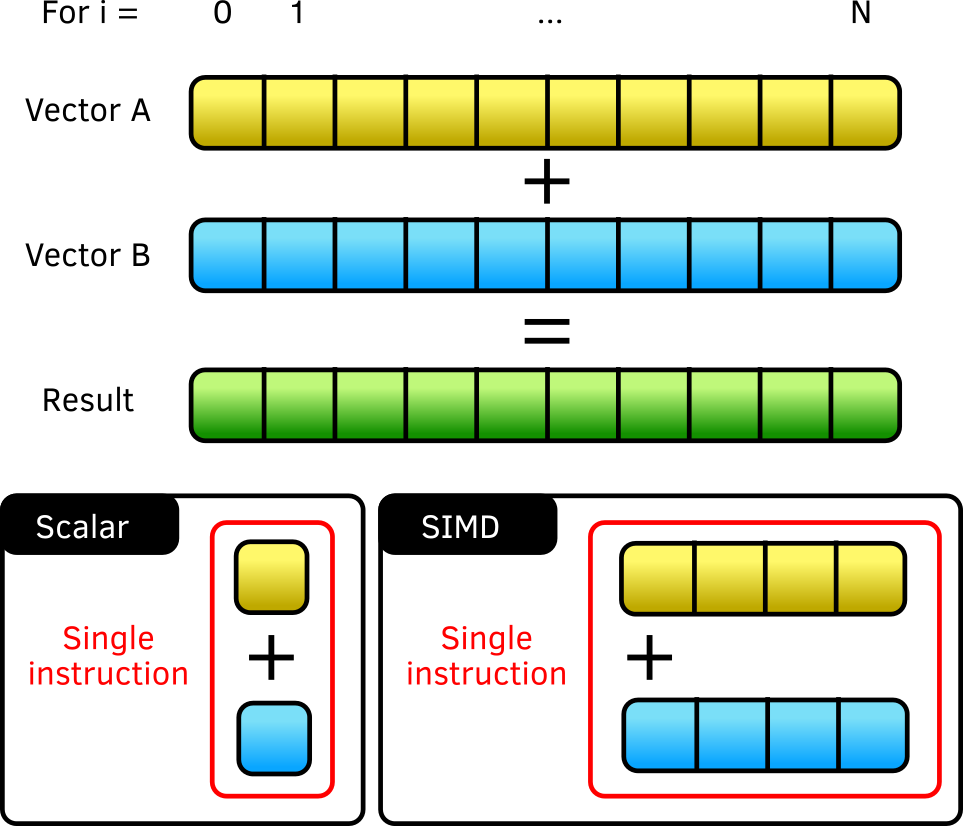
\includegraphics[width=\textwidth]{scalar_vs_SIMD.png}
        \end{column}
        \begin{column}{0.5\linewidth}
            \begin{itemize}
                \item Modern CPUs have instructions capable of doing multiple computations at the same time (e.g. do 4 distinct additions with a single instruction)
                \item SIMD: \structure{S}ingle \structure{I}nstruction \structure{M}ultiple \structure{D}ata
                \item Can get up to $M$ times faster with SIMD units of size $M$
            \end{itemize}
        \end{column}
    \end{columns}
\end{frame}

\begin{frame}[fragile]{What is vectorization}
    \begin{itemize}
        \item To vectorize, we use special functions called \structure{intrinsics}
        \item These are functions provided by the compiler
        \item They map to hardware instructions
        \item SIMD intrinsics are only portable between CPUs using the same instruction set:
        \begin{itemize}
            \item x86 $\rightarrow$ SSE, AVX
            \item ARM $\rightarrow$ NEON, SVE
            \item RISC-V $\rightarrow$ RVV
            \item ...
        \end{itemize}
    \end{itemize}
\end{frame}

\begin{frame}[fragile]{Example: usage of SIMD intrinsics}
    For example, adding two SIMD vectors of \texttt{double} using intrinsics:
    \begin{columns}
        \begin{column}{0.5\linewidth}
            \begin{center}
                \caption{Using AVX2 (Intel, AMD CPUs)}
                \begin{minted}{C++}
                    #include <immintrin.h>

                    __m256d a, b;
                    a = _mm256_add_pd(a, b);
                \end{minted}
            \end{center}
        \end{column}
        \begin{column}{0.5\linewidth}
            \begin{center}
                \caption{Using SVE (ARM CPUs)}
                \begin{minted}{C++}
                    #include <arm_sve.h>

                    svfloat64_t a, b;
                    a = svadd_m(svptrue_b64(), a, b);
                \end{minted}
            \end{center}
        \end{column}
    \end{columns}

    \vspace{10pt}

    We run into \structure{two problems}:
    \begin{enumerate}
        \item Writing code using intrinsics is not portable
        \item Writing code for each instruction set is repetitive and time-consuming
    \end{enumerate}
\end{frame}

\begin{frame}[fragile]{What about auto-vectorization?}
    \begin{columns}
        \begin{column}{0.5\linewidth}
            \begin{itemize}
                \item With the right flags, compilers can vectorize some parts of your code
                \item Not a solution to our problem, since vectorization is not guaranteed
                \item Sometimes the code is too complex for the compiler to vectorize (aliasing, dependencies, ...)
                \item \texttt{\#pragma ivdep} or \texttt{\#pragma omp simd} can help, but we cannot put pragmas on a Kokkos parallel loop
            \end{itemize}
        \end{column}
        \begin{column}{0.5\linewidth}
            \begin{minted}{C++}
                #pragma ivdep
                for (int i = 0; i < m; i++)
                    a[i] = a[i + k] * c;
            \end{minted}
            \begin{minted}{C++}
                Kokkos::parallel_for("loop", m,
                    KOKKOS_LAMBDA(int i) {
                        a(i) = a(i + k) * c;
                    }
                );
            \end{minted}
        \end{column}
    \end{columns}
\end{frame}

\begin{frame}[fragile]{Vectorization libraries}
    \structure{Solution:} vectorization libraries

    \vspace{10pt}

    They offer:
    \begin{itemize}
        \item Higher level types and functions to manipulate vectors
        \item A C++ API to the SIMD intrinsics
        \item A portable abstraction over the platform specific intrinsics
    \end{itemize}
\end{frame}

\begin{frame}[fragile]{Vectorization libraries: Kokkos SIMD}
    \begin{columns}
        \begin{column}{0.4\linewidth}
            Kokkos comes with a vectorization library: \structure{Kokkos SIMD}
            \begin{itemize}
                \item Specific header
                \item The platform specific vector type is abstracted away
                \item We use regular C++ operators to manipulate vectors
            \end{itemize}
        \end{column}
        \begin{column}{0.6\linewidth}
            \begin{center}
                \caption{AVX2}
                \begin{minted}{C++}
                    #include <immintrin.h>

                    __m256d a, b;
                    a = _mm256_add_pd(a, b);
                \end{minted}
            \end{center}
            \begin{center}
                \caption{Kokkos SIMD}
                \begin{minted}{C++}
                    #include <Kokkos_SIMD.hpp>

                    Kokkos::Experimental::simd<double> a, b;
                    a += b;
                \end{minted}
            \end{center}
        \end{column}
    \end{columns}
\end{frame}

\begin{frame}[fragile]{Vectorization libraries: C++ standard SIMD}
    \begin{itemize}
        \item The C++26 standard will include SIMD facilities
        \begin{minted}{C++}
            std::simd<double> x;
        \end{minted}
        \item Kokkos SIMD follows the same API
        \item It solves the portability between CPUs
        \item But Kokkos requires portability between CPU and GPU
        \item Using vectorized CPU instructions on the GPU is not possible \\
        We will see later how Kokkos handles this
    \end{itemize}
\end{frame}

\begin{frame}[fragile]{What Kokkos SIMD provides}
    \begin{itemize}
        \item A \texttt{Kokkos::Experimental::simd} type wrapping platform specific vectors
        \item A corresponding \texttt{Kokkos::Experimental::simd\_mask} type
        \item Operators for doing basic operations on these types (arithmetic, bitwise, shift, comparison, ...), which allows for more readable code
        \begin{minted}{C++}
            Kokkos::Experimental::simd<int> a, b, c;
            a *= (a + b) & (c << 2);
        \end{minted}
        \item Auxiliary functions (load, store, etc)
        \item Math functions working on SIMD types
    \end{itemize}

    \vspace{-0.75em}

    \begin{block}{Compiling Kokkos for vectorization}
        In order to enable vectorization, you should specify a CPU architecture flag with cmake, or use \texttt{-DKokkos\_ARCH\_NATIVE=ON} to optimize for the CPU you are compiling on
    \end{block}
\end{frame}

\begin{frame}[fragile]{Kokkos SIMD}
    \begin{itemize}
        \item Kokkos SIMD supports the following datatypes: \texttt{float}, \texttt{double}, \texttt{int32\_t}, \texttt{uint32\_t}, \texttt{int64\_t}, \texttt{uint64\_t}
        \item \texttt{Kokkos::Experimental::simd<T>} will default to the vector type with the largest size for type \texttt{T}
        \item You can also explicitly request a size: \texttt{Kokkos::Experimental::simd<float, N>}\\
        Be careful, different platforms have different vector sizes
        \item If needed, you can also directly specify an abi: \texttt{Kokkos::Experimental::basic\_simd<float, abi>}
    \end{itemize}
    \begin{block}{SIMD abi}
        In Kokkos SIMD, abis are types used to identify an instruction set and a vector length. Using an abi directly is \structure{not portable}.
    \end{block}
\end{frame}

\begin{frame}[fragile]{Supported SIMD abis}
    \begin{center}
        \begin{table}{SIMD abis}{lll}
            ISA & abi & Compatible datatypes \\\hline
            - & \texttt{scalar} & all \\
            AVX2 & \texttt{avx2\_fixed\_size<4>} & all \\
            AVX2 & \texttt{avx2\_fixed\_size<8>} & \texttt{float}, \texttt{int32\_t}, \texttt{uint32\_t} \\
            AVX512 & \texttt{avx512\_fixed\_size<8>} & all \\
            AVX512 & \texttt{avx512\_fixed\_size<16>} & \texttt{float}, \texttt{int32\_t}, \texttt{uint32\_t} \\
            NEON & \texttt{neon\_fixed\_size<2>} & all \\
            NEON & \texttt{neon\_fixed\_size<4>} & \texttt{float}, \texttt{int32\_t}, \texttt{uint32\_t} \\
            SVE & \texttt{sve\_fixed\_size<N/2>} & \texttt{double}, \texttt{int64\_t}, \texttt{uint64\_t}, \texttt{int32\_t} \\
            SVE & \texttt{sve\_fixed\_size<N>} & \texttt{float}, \texttt{int32\_t}, \texttt{uint32\_t} \\
        \end{table}
    \end{center}
\end{frame}

\begin{frame}[fragile]{Initializing a vector}
    \begin{itemize}
        \item Default construction: the values will be uninitialized
        \vspace{-5pt}
        \begin{minted}{C++}
            Kokkos::Experimental::simd<double> x;
        \end{minted}
        \item Set every element to the same value
        \vspace{-5pt}
        \begin{minted}{C++}
            Kokkos::Experimental::simd<double> x(5.);
        \end{minted}
        \item Set each value individually
        \vspace{-5pt}
        \begin{minted}{C++}
            Kokkos::Experimental::simd<double>
                x([](int idx) { return idx * idx; });
        \end{minted}
        \item Load the values from memory
        \vspace{-5pt}
        \begin{minted}{C++}
            Kokkos::Experimental::simd<double>
                x(ptr, Kokkos::Experimental::simd_flag_default);
        \end{minted}
    \end{itemize}
\end{frame}

\begin{frame}[fragile]{Vectorizing a loop}
    A loop typically has the following structure:
    \begin{minted}{C++}
        Kokkos::parallel_for("loop", N,
            KOKKOS_LAMBDA(int i) {
                // load input data
                // do some computation
                // store the result
            }
        );
    \end{minted}

\end{frame}

\begin{frame}[fragile]{Vectorizing a loop}
    A vectorized loop follows the same pattern:
    \begin{minted}{C++}
        Kokkos::parallel_for("vectorized loop", N / VEC_WIDTH,
            KOKKOS_LAMBDA(int i) {
                // load input data into vectors
                // do some computation
                // store the result vector in memory
            }
        );
    \end{minted}
    \begin{block}{Note}
        We iterate from 0 to \texttt{N / VEC\_WIDTH}, since we compute \texttt{VEC\_WIDTH} elements per iteration
    \end{block}
\end{frame}

\begin{frame}[fragile]{Example: adding two views}
    Let's start with a simple kernel adding two views
    \begin{minted}{C++}
        Kokkos::View<double*> A("A", N);
        Kokkos::View<double*> B("B", N);
        Kokkos::parallel_for("add", N,
            KOKKOS_LAMBDA(int i) {
                A(i) += B(i);
            }
        );
    \end{minted}
\end{frame}

\begin{frame}[fragile]{Example: adding two views}
    The vectorized version is as follows
    \begin{minted}{C++}
        namespace KE = Kokkos::Experimental;
        using simd_type = KE::simd<double>;
        Kokkos::parallel_for("add", N / simd_type::size(),
            KOKKOS_LAMBDA(int i) {
                std::size_t idx = i * simd_type::size();
                // load the values
                simd_type a(&A(idx), KE::simd_flag_default);
                simd_type b(&B(idx), KE::simd_flag_default);
                // perform the computation
                a += b;
                // store the result
                KE::simd_unchecked_store(a, &A(idx), KE::simd_flag_default);
            }
        );
    \end{minted}
\end{frame}

\begin{frame}{Strategy for the Gray Scott}
    The Gray Scott is a 2D problem:
    \begin{itemize}
        \item Simplification: only consider the case where n\_columns is a multiple of the SIMD width
        \item Identify the contiguous dimension
        \item Update the iteration space relative to the contiguous dimension and compute the index
        \item Construct SIMD objects from pointers of arrays \texttt{u} and \texttt{v}
    \end{itemize}
\end{frame}

\begin{exerciseframe}{From your worktree or the "cpu" folder}
\begin{columns}
    \begin{column}{0.5\linewidth}
        \begin{minted}{C++}
            #include <Kokkos_SIMD.hpp>

            // ...

            using KE = Kokkos::Experimental;
            using simd_type = KE::simd<real>;

            View a("A", N, M);
            simd_type a_simd(&a(0, 0));
        \end{minted}
    \end{column}
    \begin{column}{0.5\linewidth}
        \begin{itemize}
            \item Duplicate your worktree folder to a different name
            \item Add the Kokkos SIMD header
            \item Use \texttt{simd} instead of scalars to compute the Gray--Scott stencil
            \item The checksum must remain the same!
        \end{itemize}
    \end{column}
\end{columns}
\end{exerciseframe}

\begin{frame}[fragile]{Conditionals (bonus)}
    \begin{itemize}
        \item Loops are not always simple
        \item Complex control flows can be problematic
        \begin{minted}{C++}
            Kokkos::parallel_for("loop", N,
                KOKKOS_LAMBDA(int i) {
                    if (A(i) > 0)
                        A(i) = Kokkos::sqrt(A(i));
                    else
                        A(i) = 0;
                }
            );
        \end{minted}
        \item We cannot use an \texttt{if} branch with a vector
        \begin{itemize}
            \item Consider the following vector \texttt{\{-1, 2, 0, 1\}}
            \item Different values of the vector would enter different branches
            \item The \texttt{condition} function, which selects values from two vectors according to a \structure{mask}
        \end{itemize}
    \end{itemize}
\end{frame}

\begin{frame}[fragile]{Masks}
    \begin{itemize}
        \item \texttt{Kokkos::Experimental::simd\_mask} acts like a vector of booleans
        \item Initialized like a \texttt{simd} vector
        \begin{minted}{C++}
            using namespace Kokkos::Experimental;
            simd_mask<double> m;       // uninitialized
            simd_mask<double> m(true); // every value is true
            // true on even indices, false on odd ones
            simd_mask<double> m(KOKKOS_LAMBDA(int i) { return i % 2 == 0; });
        \end{minted}
        \item This is the type returned by comparison operations
        \begin{minted}{C++}
            Kokkos::Experimental::simd<double> x;
            Kokkos::Experimental::simd_mask<double> m = x > 0.;
        \end{minted}
        \item They can be used in the \texttt{condition} function, to conditionally load/store elements of a vector or in reduction operations
    \end{itemize}
    \vspace{0.5em}
\end{frame}

\begin{frame}[fragile]{Example: vectorizing with conditionals}
    Here is a kernel computing $a = \sqrt{a}$ if $a$ is positive, or $a = 0$ otherwise
    \begin{minted}{C++}
        Kokkos::View<double*> A("A", N);
        Kokkos::parallel_for("sqrt", N,
            KOKKOS_LAMBDA(int i) {
                if (A(i) > 0)
                    A(i) = Kokkos::sqrt(A(i));
                else
                    A(i) = 0.;
            }
        ):
    \end{minted}
\end{frame}

\begin{frame}[fragile]{Example: vectorizing with conditionals}
    Here is the vectorized version
    \begin{minted}{C++}
        using simd_type = Kokkos::Experimental::simd<double>;
        Kokkos::parallel_for("sqrt", N / simd_type::size(),
            KOKKOS_LAMBDA(int i) {
                std::size_t idx = i * simd_type::size();
                simd_type a(&A(idx), Kokkos::Experimental::simd_flag_default);
                a = Kokkos::Experimental::condition(a > 0, Kokkos::sqrt(a), 0.);
                Kokkos::Experimental::simd_unchecked_store(a, &A(idx), Kokkos::Experimental::simd_flag_default);
            }
        );
    \end{minted}

    \vspace{-1em}
    \begin{columns}
        \begin{column}{0.8\linewidth}
            \begin{block}{Observation}
                \texttt{condition} takes a \texttt{simd\_mask}, and two vectors, and selects elements from both vectors depending on the values in the mask
            \end{block}
        \end{column}
        \begin{column}{0.2\linewidth}
            \begin{block}{Note}
                Both branches are evaluated
            \end{block}
        \end{column}
    \end{columns}
\end{frame}

\section{Conclusion}

\begin{frame}{Conclusion}
    \begin{itemize}
        \item Kokkos provides views as useful data containers
        \item \texttt{parall\_for} and \texttt{parallel\_reduce} for parallel constructs
        \item \texttt{RangePolicy} and \texttt{MDRangePolicy} for loop dimensionality
        \item CPU optimization with SIMD
    \end{itemize}
    \pause
    \vspace{2em}
    \begin{alertblock}{Caution}
        The Kokkos code so far only works on CPU and is not portable! We will make it portable next week
    \end{alertblock}
\end{frame}

\begin{frame}[plain]
    \closingpage
\end{frame}

\end{document}
